\documentclass[a4paper,12pt]{article}
\usepackage[toc,page]{appendix}
\usepackage{listings}
\usepackage{url}
\usepackage{graphicx}
\usepackage[skip=0pt]{caption}
\usepackage{multicol}
\usepackage{float}
\usepackage[margin=1in]{geometry}
%\usepackage{natbib}

\begin{document}

\renewcommand{\thelstlisting}{\thesection.\arabic{lstlisting}}
\renewcommand{\thefigure}{\arabic{section}.\arabic{figure}}
\renewcommand{\thetable}{\arabic{section}.\arabic{table}}
\setlength{\floatsep}{0pt plus 2pt minus 2pt}
%\setlength{\intextsep}{0pt plus 2pt minus 2pt}
%\setlength{\textfloatsep}{0pt plus 2pt minus 2pt}

\title{Introduction to Digital Libraries Assignment \#4}
\date{April 23, 2015}
\author{James Tate II}
\maketitle

\section{Introduction}
Assignment \#4 first required analyzing the changes (if any) in the representations retrieved
in assignment \#3. The same URIs were dereferenced again and compared to the previous
representations. The next part of this assignment involved retrieving TimeMaps of the
analyzed URIs, and analyzing the number of mementos each URI had. The last part of the
assignment required generating graphs of Jaccard Distance over time of 20 URIs.

\section{Methodology}
I wrote several scripts for this assignment and I also modified some previously-written
scripts. They are described in subsections for the different questions in this assginment.

\subsection{Question \#1}
The first part of Question \#1 was to again dereference the URIs that were successfully
processed by boilerpipe in Assignment \#3\cite{hw3}. I used the command in Listing 2-1 to
get a list of the dereferenced URIs that were successfully processed in Assignment \#3.

\begin{lstlisting}[basicstyle=\ttfamily,caption={Getting URIs that
Succeded Boilerpipe Processing }]
    grep -v " 0 " wc_boilerpipe | awk4 \
      | grep -o "\./tweets/[0-9]\+/" \
      > boilerpipe_success_dirs
\end{lstlisting}

Next, I created a new directory to store the second representations of the URIs. I populated
the directory will the URI files I would need to dereference the URIs. These steps are in
Listing 2.2.

\begin{lstlisting}[basicstyle=\ttfamily,caption={Creating Second Tweets Directory}]
    mkdir tweets2
    for i in $(cat boilerpipe_success_dirs);
      do id=$(echo $i | grep -o "[0-9]\+");
      mkdir tweets2/$id;
      cp "${i}url.0" tweets2/$id/url.0;
    done
\end{lstlisting}

I then dereferenced the URIs using the same script from Assignment \#1 which I modified to
used the new directory\cite{hw1}. This step is shown in Listing 2.3. It took 136 seconds to dereference
3035 URIs using 128 parallel processes. 146 did not dereference successfully. The first dereference in
Assignment \#1 was on February 11. The second dereference in this assignment was on April 22, a difference
of 70 days.

\begin{lstlisting}[basicstyle=\ttfamily,caption={Dereferencing URIs}]
    ./dereference_URIs.py
\end{lstlisting}

After obtaining new representations, I created a list of downloaded represenations and processed the files
with boilerpipe, as shown in Listing 2.4.

\begin{lstlisting}[basicstyle=\ttfamily,caption={Extracting Text with Boilerpipe}]
    find ./tweets2/ > tweets2_file_list
    ./run_boilerpipe.py
\end{lstlisting}

Once I had the textual output from boilerpipe I was ready to start the processing with my \emph{jaccard.py}
script. This script removes most punctuation from the text, generates sets of unigrams, bigrams and trigrams
then calculates the Jaccard Distance between the two representations of each resource\cite{wiki:jaccard}.
These commands to
setup input lists for my script and to run in are in Listing 2.5. The first four commands removed
URIs with a second representation that was not successfuly processed by boilerpipe.

\begin{lstlisting}[basicstyle=\ttfamily,caption={Calculating Jaccard Distance}]
  wc tweets2/*/*/boilerpipe.output | tee wc_boilerpipe2
  grep -v "^ \+0 " wc_boilerpipe | grep -v " total$" \
    | awk4 | grep -o "56[0-9]\+" > boilerpipe1_ids
  grep -v "^ \+0 " wc_boilerpipe2 | grep -v " total$" \
    | awk4 | grep -o "56[0-9]\+" > boilerpipe2_ids
  comm -12 <(sort boilerpipe1_ids) <(sort boilerpipe2_ids) \
    > boilerpipe_common_ids
  ./jaccard.py | tee hw4_report/stats/q1_distances.stats
\end{lstlisting}

The last step for this question was to generate three files for consumption by R to make the graphs in the
Results section. These files were generated by the commands in Listing 2.6.

\begin{lstlisting}[basicstyle=\ttfamily,caption={Generating R Input Files}]
    awk2 q1_distances.stats | tail -n +2 \
      | sort -n > q1_unigrams.stats
    awk3 q1_distances.stats | tail -n +2 \
      | sort -n > q1_bigrams.stats
    awk4 q1_distances.stats | tail -n +2 \
      | sort -n > q1_trigrams.stats
\end{lstlisting}

\subsection{Question \#2}
Question \#2 required me to download the TimeMaps for each URI, and count how many Mementos each URI had.
I made a script, \emph{get\_timemaps.py}, and used it to download the TimeMaps as shown is Listing 2.7.

\begin{lstlisting}[basicstyle=\ttfamily,caption={Downloading TimeMaps}]
    ./get_timemaps.py > get_timemap_output
\end{lstlisting}

This script downloads TimeMapIndexes from the \emph{Time Travel} service on mementoweb.org. The
TimeMapIndexes contain links to TimeMaps from several different providers, which were subsequently
downloaded. All the downloaded files were stored in a ``timemaps'' subdirectory of the URI's content
directory.

The next step was to count the Mementos available for each URI. This was done using a long pipeline of
shell commands, and another Python script, \emph{count\_mementos.py}. Listing 2.8 shows both of these
commands.

\begin{lstlisting}[basicstyle=\ttfamily,caption={Counting Mementos}]
    find ./tweets2/ > tweets2_file_list
    grep "\.timemap$" tweets2_file_list \
      | xargs grep memento \
      | grep -v rel=\"timemap\" \
      | grep -v rel=\"timegate\" \
      | grep -v rel=\"self\" \
      | tee memento_list
    ./count_mementos.py > memento_counts
\end{lstlisting}

\subsection{Question \#3}



\section{Results}
This section is broken into subsections for each question.

\subsection{Question \#1}
The Jaccard Distance of the representations was zero for about four-fifths of the representations. This means
most representations did not change between the times I dereferenced their URIs. Of the remaining fifth,
there was a mix of pages that changed a little, changed a lot and were completely different. Only the
when considering the Jaccard Distance of trigrams, did any pages score 1.0. A 1.0 Jaccard Distance means
the two representations did not have any n-grams in common.

I excluded representations that did not have any output from boilerpipe in these results. One effect of that
exclusion is webpages that were not available at the time of the second dereference are not included in the
results. The URIs would have generally scored high Jaccard Distances, skewing the results.

Figures 3.1 through 3.3 show the Cumulative Distribution Function plot of the calculated Jaccard Distances
for the different n-grams.

\begin{figure}[H]
    \centering
    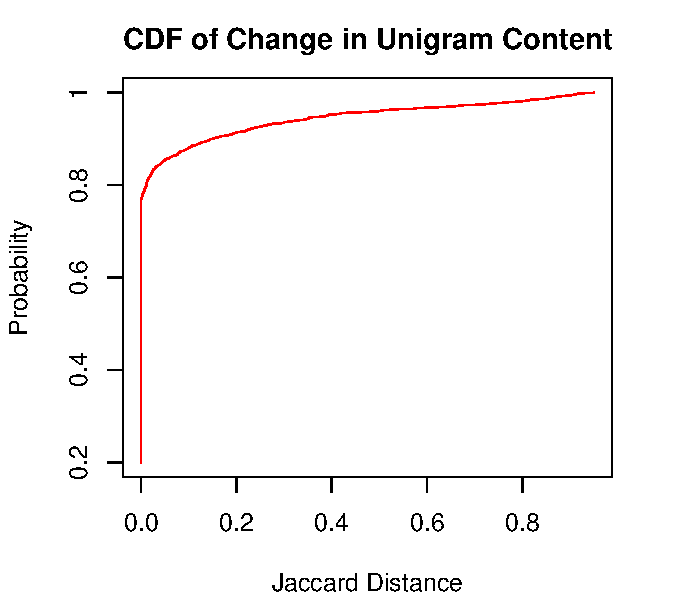
\includegraphics{stats/q1_unigrams.pdf}
    \caption{Unigram Jaccard Distance}
\end{figure}
\begin{figure}[H]
    \centering
    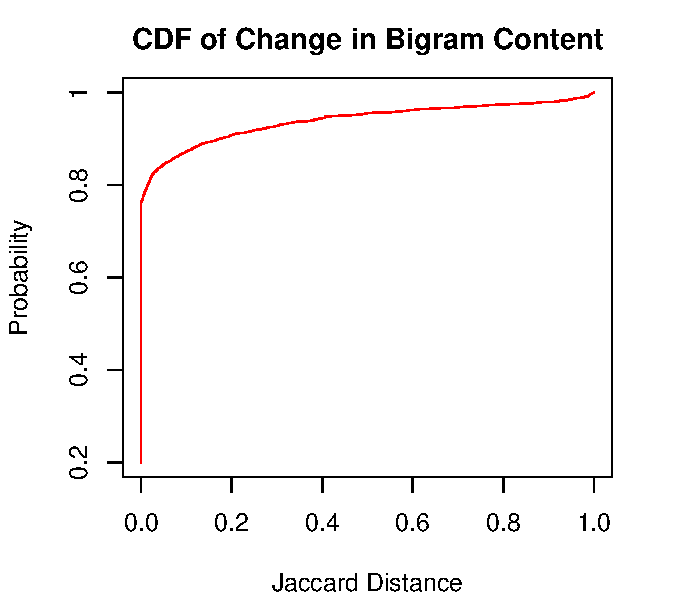
\includegraphics{stats/q1_bigrams.pdf}
    \caption{Bigram Jaccard Distance}
\end{figure}
\begin{figure}[H]
    \centering
    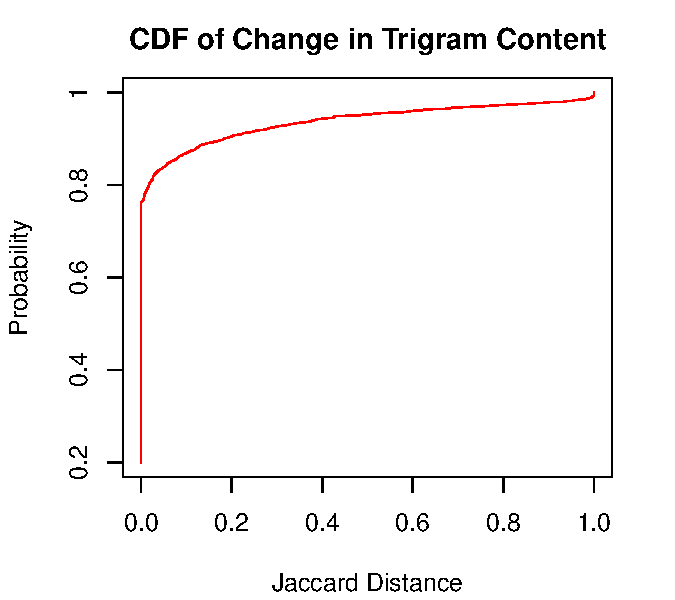
\includegraphics{stats/q1_trigrams.pdf}
    \caption{Trigram Jaccard Distance}
\end{figure}

Table 3.1 shows the Jaccard Distances for three example resources, and the average of all sampled resources.
The first resource is a \emph{USA Today} article about the measles vaccine in California. The article content
did not change at all between the two downloaded representations, so the Jaccard Distances are all 0.0.

The
second resource is the homepage of a website that offers detailed tips for making your business successful.
The page appears to list the most recent tips and only lists 10 on the homepage. During the gap between when
the two representations were downloaded, six new tips were added to the list, which pushed off six older tips,
explaining the about 0.6 Jaccard Distance in the three n-gram categories.

The third example resource is the homepage of a US-based Nigerian news website. There do not appear to be any
of the same articles described on the homepage between the two representations, which explains the near 1.0
Jaccard distances. The boilerpipe output for the first and second representations of the three example
resources is in Appendix A.

The average Jaccard Distances in the last row of Table 3.1 show higher distances for greater values of
\emph{n}. This pattern was seen on every individuals resource on which I examined the scores.
Presumably it is easier for two documents to have a lower Jaccard Distance when fewer elements are
grouped together in the n-grams.

\begin{table}[H]
\centering
\caption{Example Jaccard Distances}
\begin{tabular}{ | c | c | c | c | }
\hline
\textbf{Resource}  & \textbf{Unigram Distance} & \textbf{Bigram Distance} & \textbf{Trigram Distance} \\ \hline
Measles Article & 0.000  & 0.000  & 0.000  \\ \hline
Business Tips   & 0.521  & 0.651  & 0.671  \\ \hline
Nigerian News   & 0.908  & 0.989  & 0.998  \\ \hline
Average         & 0.066  & 0.076  & 0.078  \\ \hline
\end{tabular}
\end{table}


\subsection{Question \#2}
Of the 2735 URIs being processed at this point, 1715 of them did not have any Mementos. Of the remaining
1020 URIs, most had a single Memento, but one had 10030 Mementos. The average number of Mementos was 19.8.
Figures 3.4 and 3.5 below show the plot of the CDF of the number of Mementos. The first graph is of all
URIs. The second is only of the URIs with a nonzero Memento count and is shown with a logarithmic scale
on the X-axis.

\begin{figure}[H]
    \centering
    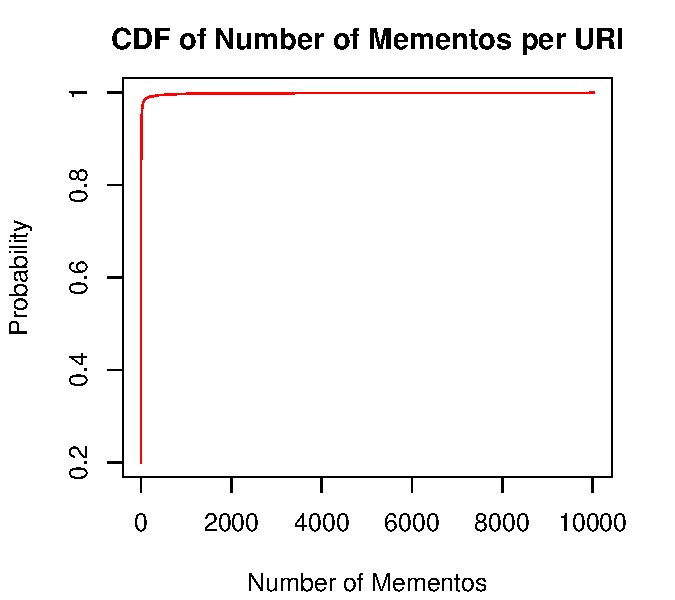
\includegraphics{stats/memento_counts.pdf}
\end{figure}

\begin{figure}[H]
    \centering
    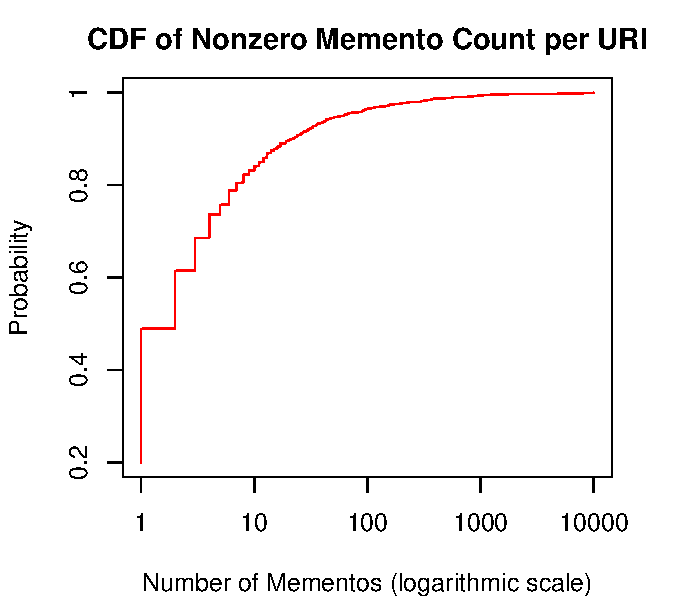
\includegraphics{stats/memento_counts_nonzero.pdf}
    %\caption{Trigram Jaccard Distance}
\end{figure}

\subsection{Question \#3}


\clearpage
\begin{appendices}
\section{Example Boilerpipe Output}
\subsection{Measles Article (February and April Representations Identical)}
Calif. school releases students unvaccinated for measles
Palm Desert High School students Jesus Vejar, left, and Isaac Perez, both 18, show a letter from the Riverside County Department of Public Health informing them of precautions being taken because of potential measles cases.(Photo: Richard Lui, The (Palm Springs, Calif.) Desert Sun)
PALM SPRINGS, Calif. âearly 70 students from a Riverside County, Calif., high school will miss up to seven days of classes because they haven't been immunized for measles.
Since the 66 Palm Desert High School students haven't been immunized, they need to avoid classes until Feb. 9 unless they confirm they've received immunization or show proof of resistance as determined by a Titer test, according to the Desert Sands Unified School District.
In 2014, the CDC reports there were 644 cases from 27 states. That is the largest number of cases since measles elimination was documented in the U.S. in 2000.
And in Arizona, health officials believe a woman who has recently been diagnosed with measles may have exposed as many as 195 children at a children's center to the disease.
Earlier this month, health officials in Orange County, Calif., where Disneyland is located, told 24 unvaccinated students to stay home for three weeks âhe incubation period for measles âfter learning that an infected student attended Huntington Beach High School.
Health officials checked all students' immunization status Tuesday after a girl was sent home Monday because of a suspected case of measles. She was later cleared to return to class Tuesday.
The 66 students didn't need to be quarantined, but they couldn't leave campus until their parents arrived to take them home.
"We need to arrange for parents to make that kind of transportation arrangement," said district spokeswoman Mary Perry. "You can't send them to the door and make them leave."
Palm Desert High School is sending 66 students who have not been vaccinated for measles home Wednesday, Jan. 28, 2015, after a suspected case of measles this week. The front of the new high school in 2011.(Photo: Jay Calderon, The (Palm Springs, Calif.) Desert Sun)
Several students said Wednesday that they weren't worried about catching the measles since they were already immunized. However, they said they felt bad for the students who were sent home.
"It's the start of a second semester. This is not a good time to be missing school," said freshman Michael Wallace.
There haven't been any reports of possible cases of measles elsewhere and "at this point, all efforts are focused on the high school," Perry said.
It wasn't immediately clear, however, why the students weren't immunized.
While all states require that children receive recommended vaccines before attending school, some make it easier than others to get exemptions. Infectious disease outbreaks are more common in areas with large numbers of unvaccinated students.
All states grant exemptions to children for medical reasons, such as immune deficiencies. And all states except Mississippi and West Virginia grant exemptions based on religious objections, according to the National Conference of State Legislatures.
Nineteen states, including California, allow students to skip vaccines for philosophical objections. Some states require vaccines only for public school students; other laws apply to public and private schools.
Nearly 95\% of children are fully vaccinated against measles, according to the CDC. But vaccination rates vary from a low of 82\% in Colorado to 98\% in Mississippi.
Measles symptoms include fever or rash, running nose, coughing and red eyes. Symptoms typically appear seven to 12 days after exposure to measles but may take up to 21 days.
Four people have been diagnosed with measles in western Riverside County, Calif., over the past month. Their cases were linked to the amusement park outbreak.
According to the Riverside County health department, there was no indication the first Palm Desert High School student recently visited Disneyland.
In a health department letter to Palm Desert parents, officials said, "Your child is at risk of developing measles if she/he has never had the disease or has not received two doses of measles vaccine. If your child has received one vaccination, she/he may not be immune and could develop measles."
Statewide, 79 California residents have been diagnosed with measles during the outbreak, according to the California Department of Public Health. Of those, 52 were connected to the exposure at Disneyland. Most of those whose vaccination status was documented had not been immunized.
Most children receive measles-mumps-rubella (MMR) vaccines at age 1 and again at age 4. Most children are protected after only one dose of the vaccine, but parents should ask doctors about receiving a second shot, according to the Riverside County health department.
\subsection{Business Tips Homepage February Representation}
What did you install and use in your PC? In internet millions of free and paid software are available to make easy to solve people problems. To make easier for you, we have created this list and make top 15 free PC programs.... Read more
Now they have more than 1 billion users worldwide. Facebook change the world, they gave lots of options for user such as sharing updates, photos and videos with family, friends and advertising option for business owner...... Read more
Computer animation refers to any sequence of visual changes in a scene, i.e. it is a series of images that are displayed in sequences. In addition to changing object position with translations or rotations, a computer generated animation.... Read more
Types of network on the basis of area are:LAN is entirely contained within a buildings, school, and college or extended up to few or 5 KM (kilometers) with wire. The wire (twisted pair, fiber optic) used in LAN must be of same type.... Read more
I saw many people's are begging for follow me on twitter Do you searching cheap best web hosting companies? There are lots of sites; some of them will be able to provide 100\% customer support, 99.99\% uptime. We collect information about web page hosts, test and web page hosting programs prices also....Read more
Every business company or organization wants register a domain name for making sales, online marketing, promotes their business in online. We can help you to find perfect domain names and setting up your website for your business....Read more
When I first start web design it is very hard to know what to do, because i was once the same as you. In this time creating websites becomes much easier and I think watching video tutorials, online courses and help with other peoples is the fastest way to learn....Read more
There are many SEO tips and tricks that should not be working and canâmake your web pages rank higher in search engines. SEO is divided into two main parts i.e. On-page SEO \& off page SEO. Both are required to do perfect search engine optimization... Read more
Learn how to make a website using web applications like PHP and MySQL, HTML, CSS, and Software like Dreamweaver, Code editors and many more. Learn web development basics like building an ecommerce site \& more advanced skills like how to... Read more
How can i help?
It is our goal to help you solutions for Social media tips and tricks, General computer Solutions, Web designing and Programming Solutions, Microsoft / Windows helps, Make money at online and many more...
\subsection{Business Tips Homepage April Representation}
Most of people create blog and website and they try to monetize with their blogs with Google AdSense. I also try this, but I am always worried about being suspended and banned from AdSense for life time..... Read more
HTML is a simple scripting language used to develop website or language. HTML file is a text file containing small markup tags. The markup tags tell the browsers how to display the page for the users..... Read more
We make Top 35 keyboard shortcuts for help and keep focus on time management or easily. We use keyboard shortcuts for highlighting text, copy, paste, open, close undo, redo and many more others. I want to give one example.... Read more
How to start at online, read this website articles it can help you. At online peoples can do everything reading, knowing important thing, news or it make peoples life much easier. If you donâhave a job you can search job at online.... Read more
What did you install and use in your PC? In internet millions of free and paid software are available to make easy to solve peopleâproblems. To make easier for you, we have created this list and make top 15 free PC programs.... Read more
Now they have more than 1 billion users worldwide. Facebook change the world, they gave lots of options for user such as sharing updates, photos and videos with family, friends and advertising option for business owner...... Read more
Computer animation refers to any sequence of visual changes in a scene, i.e. it is a series of images that are displayed in sequences. In addition to changing object position with translations or rotations, a computer ânerated animation.... Read more
Types of network on the basis of area are:LAN is entirely contained within a buildings, school, and college or extended up to few or 5 KM (kilometers) with wire. The wire (twisted pair, fiber optic) used in LAN must be of same type.... Read more
How can i help?
It is our goal to help you solutions for Social media tips and tricks, General computer Solutions, Web designing and Programming Solutions, Microsoft / Windows helps, Make money at online and many more...
\subsection{Nigerian News Homepage February Representation}
Breaking News
The Economist Nigeria's electionThe EconomistSOMETIMES there are no good options. Nigeria goes to the polls on February 14th to elect the next president, who will face problems so largeâom rampant corruption to a jihadist insurgencyy that they could break the country apart, with dire The real reason Nigeria should delay electionsAl Jazeera AmericaBid to Delay Nigeria's
Wall Street Journal Oil futures turn higher in volatile trade after heavy lossesNasdaqThe U.S. Energy Information Administration said that U.S. crude oil inventories rose by 6.3 million barrels last week to 413.1 million, the most in records dating back to August 1982. West Texas Intermediate oil futures rose nearly 19\% in the four Oil prices
Ads:
9ja News
The Economist Nigerian politicsThe EconomistA THREE-CAR convoy is considered modest for leading Nigerian politicians, and modesty appeals to Muhammadu Buhari, the leading opposition candidate in the presidential election due to be held on February 14th. From his rented house made of simple Who Will Choose Nigeria's Next President?The New YorkerThe real reason Nigeria should delay electionsAl
Straight.com Gwynne Dyer: Nigeria's troubled presidential electionStraight.comNigeria's president, Goodluck Jonathan, has lived up to his name again. Three minutes after he left an election rally in the northern city of Gombe on Monday, a suicide bomber blew herself up in the nearby parking lot. The president had just passed PHOTOS: KSB meets Buhari, Osinbajo, othersNigerian
BBC News Chad Retakes Nigerian Town From Militant Group Boko HaramNew York TimesABUJA, Nigeria \& Chad's government said this week that its military had retaken a border town in Nigeria from the Islamist militant group Boko Haram, suggesting that momentum in the nearly six-year war against the group may finally be shifting. Chad Boko
Nigerian Entertainment Today Paul Adefarasin's HOTR brings 'Selma' to NigeriaNigerian Entertainment TodayThe House On The Rock Church led by top Nigerian minister, author and social transformer, Paul Adeolu Adefarasin, is set to bring the 2014 American blockbuster, Selma to its members as well as those interested in the movie in Nigeria. According to And more
Moneycontrol.com WTI oil futures extend losses after plunging 9\% on WednesdayNasdaqInvesting.com Crude oil futures extended sharp losses from the previous session on Thursday, as fears over a glut in supplies intensified after data showed that oil supplies in the U.S. rose to the highest level on record last week. On the New York Crude
\subsection{Nigerian News Homepage Representation}
Nigerian Entertainment Conference: Alex Okosi, Lagbaja, Tony Okoroji Pulse NigeriaThe third edition of the Nigerian Entertainment Conference (NECLive) holding On Wednesday April 22, 2015 at the Eko Hotel and Suites in Lagos, will be respecting contributors to Nigerian show business with the NET Honours, this award is in recognition nigeria entertainment news Google News \[...\]
BBC Sport Nigeria appoint Stephen Keshi for third timeBBC Sport"To succeed we all need to come together as one because Nigeria belongs to us, this is not Stephen Keshi's team but our national team." BBC Sport understands that Keshi has been set several targets and that his contract will be terminated if he does âtephen Keshi signs new contract as Nigeria coachWashington TimesBREAKING: Stephen Keshi signs new Nigeria contractGoal.comNigeria's Keshi saga endsSport24all 80 news articles Nigeria Google News \[...\]
CTV News Stephen Keshi signs 2-year contract as coach of Nigeria's national soccer teamCTV NewsABUJA, Nigeria âtephen Keshi signed a two-year contract to continue as head coach of Nigeria on Tuesday, calling it "a new page" after a tumultuous story so far that has seen him guide the country to the African title, resign, return, get fired and âtephen Keshi signs new contract as Nigeria coachHilton Head Island PacketKeshi signs two-year extension as Nigeria coachThe West Australianall 78 news articles nigeria soccer Google News \[...\]


\end{appendices}

%\begin{figure}[H]
%    \centering
%    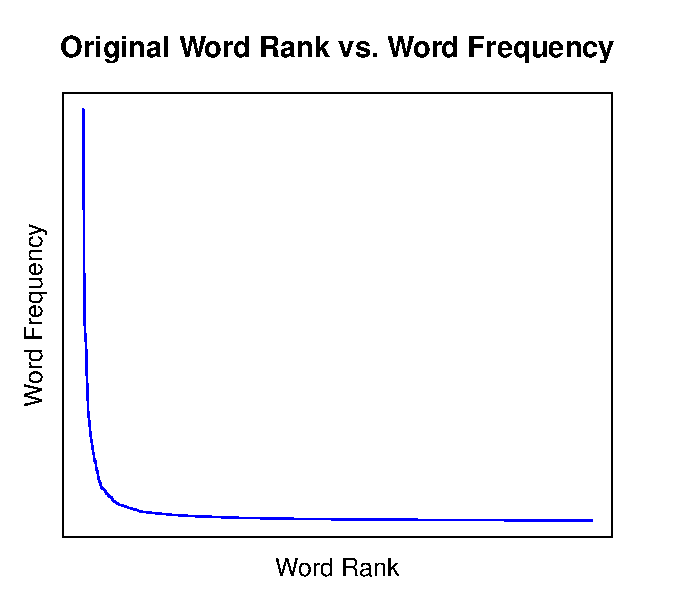
\includegraphics{stats/original_words.pdf}
%    \caption{Rank of Original Words vs. Their Frequency}
%\end{figure}

\clearpage
\bibliographystyle{plain}
\bibliography{../../cs751}

\end{document}
